\documentclass{beamer}

\usepackage[utf8]{inputenc}
\usepackage[english]{babel}
\usepackage{etex}
\usepackage{graphicx}
\usepackage{color}
\usepackage{hyperref}
\usepackage{verbatim}
\usepackage{url}
\usepackage{moreverb}
\usepackage{fancyvrb}
\usepackage{natbib}
\usepackage{eulervm}
\usepackage{auto-pst-pdf}
\usepackage{pst-plot}
\usepackage{amssymb}
\usepackage{pifont}
\usepackage{algpseudocode}
\usepackage{multirow}

% Code snippets
\usepackage{minted}
\definecolor{rulecolor}{rgb}{0.80,0.80,0.80}
\definecolor{bgcolor}{rgb}{1.0,1.0,1.0}
\newminted{python}{bgcolor=bgcolor}

% Checked marks
\newcommand{\cmark}{\ding{51}}%
\newcommand{\xmark}{\ding{55}}%

% Colors
\newrgbcolor{mygreen}{.00 .5 .00}
\newcommand{\X}[1]{\textcolor{blue}{#1}}
\newcommand{\y}[1]{\textcolor{red}{#1}}
\newcommand{\model}[1]{\textcolor{mygreen}{#1}}
\newcommand{\loss}[1]{\textcolor{lightblue}{#1}}

% Beamer layout
\hypersetup{colorlinks=true, linkcolor=black, urlcolor=blue}
\usetheme{boxes}
\beamertemplatenavigationsymbolsempty
\setbeamertemplate{sections/subsections in toc}[circle]
\setbeamertemplate{footline}[frame number]
\setbeamertemplate{itemize items}[circle]
\setbeamertemplate{itemize subitem}[square]

% Front slide
\title{{\bf Tree models with Scikit-Learn}\\
Great learners with little assumptions}
\author{
Material: \url{https://github.com/glouppe/talk-pydata2015}\\
\vspace{1cm}
Gilles Louppe (\href{https://twitter.com/glouppe}{@glouppe})\\
{\it CERN}
}
\date{PyData, April 3, 2015}

% Argmax
\DeclareMathOperator*{\argmax}{arg\,max}

\begin{document}

\begin{frame}
\titlepage
\end{frame}


% Random things to talk about:
% - class_weights
% - oob samples
% - n_jobs


% Outline =====================================================================

\begin{frame}
  \frametitle{Outline}
  %\tableofcontents
  \setbeamertemplate{enumerate items}[circle]
  \begin{enumerate}
  \item Motivation

  \vspace{0.5cm}

  \item Growing decision trees

  \vspace{0.5cm}

  \item Random forests

    \vspace{0.5cm}

  \item Boosting

  \vspace{0.5cm}

  \item Reading tree leaves

  \vspace{0.5cm}

  \item Summary
  \end{enumerate}
\end{frame}


% Motivation ==================================================================

\section{Motivation}

\begin{frame}
    \frametitle{Motivation}
    \begin{figure}
    \vspace{-0.5cm}
    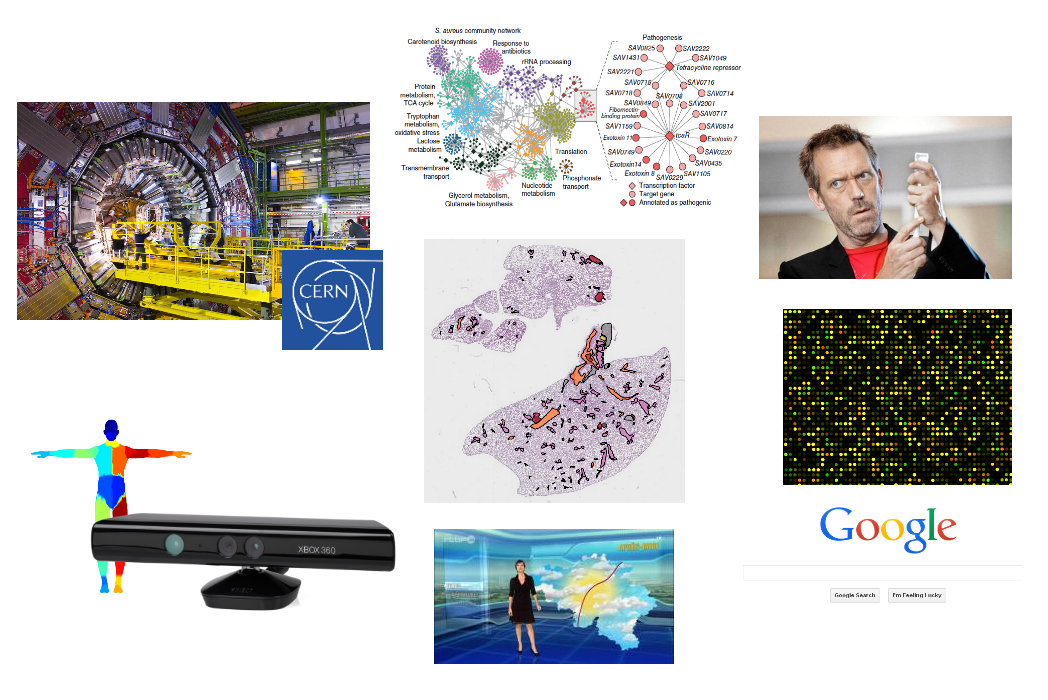
\includegraphics[scale=0.4]{./figures/motivation.png}
    \end{figure}
\end{frame}

\begin{frame}
    \frametitle{Running example}

    \begin{columns}
    \begin{column}{0.5\textwidth}

    \begin{center}
    From {\bf \X{physicochemical properties}} (alcohol, acidity, sulphates, ...),

    \vspace{1cm}
    learn a {\bf \model{model}}
    \vspace{1cm}

    to predict {\bf \y{wine taste preferences}}.

    \end{center}

    \end{column}
    \begin{column}{0.5\textwidth}
      \begin{figure}
      \vspace{-0.5cm}
      
\includegraphics[scale=0.6]{./figures/wine.jpg}
      \end{figure}
    \end{column}
    \end{columns}
\end{frame}


% Growing decision trees ======================================================

\AtBeginSection[]
{
\begin{frame}
  \frametitle{Outline}
  \tableofcontents[currentsection]
  % Die Option [pausesections]
\end{frame}
}

\section{Growing decision trees}

\begin{frame}[fragile]
    \frametitle{Supervised learning}

    \begin{itemize}
    \item Data comes as a finite learning set ${\cal L} = \texttt{(\X{X}, \y{y})}$ where
        \begin{itemize}
            \item \X{Input samples} are given as an array of shape \texttt{(n\_samples, n\_features)}\\
            \vspace{0.25cm}
            E.g., feature values for wine physicochemical properties:
\begin{verbatim}
# fixed acidity, volatile acidity, ...
X = [[  7.4    0.     ...   0.56   9.4    0.  ]
     [  7.8    0.     ...   0.68   9.8    0.  ]
                      ...
     [  7.8    0.04   ...   0.65   9.8    0.  ]]
\end{verbatim}
\vspace{0.25cm}

            \item \y{Output values} are given as an array of shape \texttt{(n\_samples,)}\\
            \vspace{0.25cm}
            E.g., wine taste preferences (from 0 to 10):
\begin{verbatim}
y = [5 5 5 ... 6 7 6]
\end{verbatim}
        \end{itemize}

    \vspace{0.25cm}

    \item The goal is to build an estimator $\model{\varphi_{\cal L}}: \X{{\cal X}} \mapsto \y{{\cal Y}}$ minimizing
    $$
    Err(\model{\varphi_{\cal L}}) = \mathbb{E}_{\X{X},\y{Y}}\{ L(\y{Y}, \model{\varphi_{\cal L}}\texttt{.predict(}\X{X}\texttt{)}) \}.
    $$
    \end{itemize}
\end{frame}

\begin{frame}[fragile]
    \frametitle{Decision trees [L. Breiman, 1984]}
    \begin{columns}
        \begin{column}{0.3\textwidth}
            \begin{figure}
            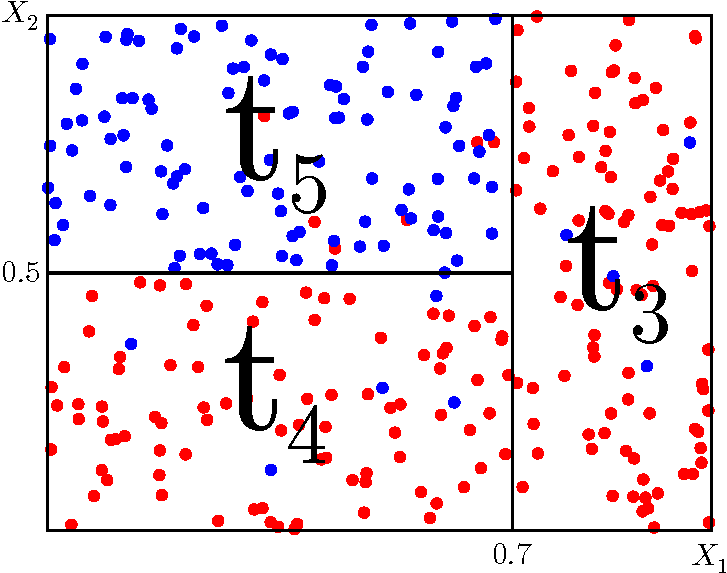
\includegraphics[width=\textwidth]{./figures/tree-partition-d.pdf}
            \end{figure}
        \end{column}
        \begin{column}{0.7\textwidth}
            \begin{figure}
            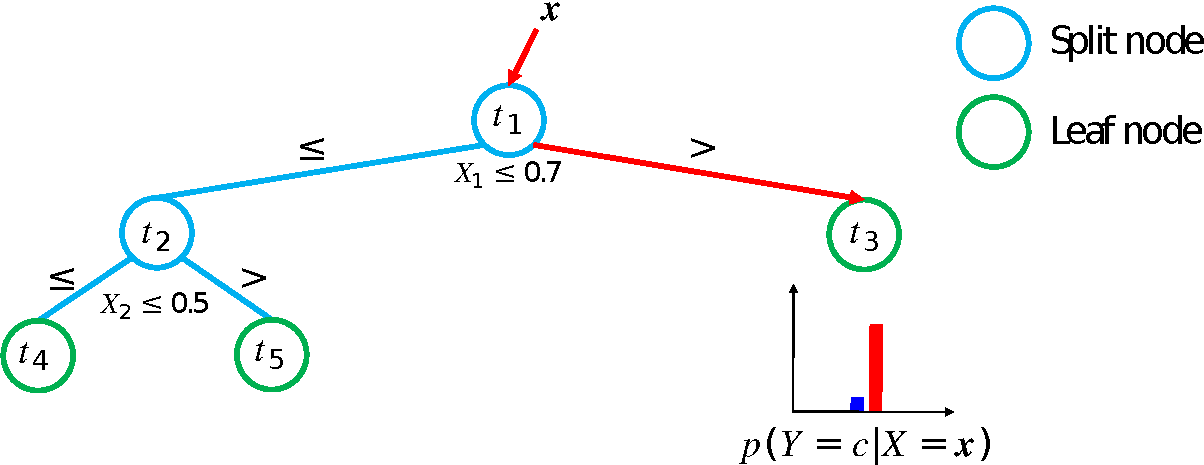
\includegraphics[width=\textwidth]{./figures/tree-simple.pdf}
            \end{figure}
        \end{column}
    \end{columns}

{\scriptsize
\begin{algorithmic}
\Function{BuildDecisionTree}{${\cal L}$}
    \State Create node $t$
    \If{the stopping criterion is met for $t$}
        \State Assign a model to $\widehat{y}_t$
    \Else
        \State Find the split on ${\cal L}$ that maximizes impurity decrease $$s^* = \argmax_{s} i(t) - p_L i(t^s_L) - p_R i(t^s_R)$$
        \State Partition ${\cal L}$ into ${\cal L}_{t_L} \cup {\cal L}_{t_R}$ according to $s^*$
        \State $t_L = \Call{BuildDecisionTree}{{\cal L}_{t_L}}$
        \State $t_R = \Call{BuildDecisionTree}{{\cal L}_{t_R}}$
    \EndIf
    \State \Return $t$
\EndFunction
\end{algorithmic}
}

\end{frame}

\begin{frame}
    \frametitle{Composability of decision trees}

    Decision trees can be used to solve several machine learning tasks by simply swapping the impurity and leaf model functions.

    \vspace{0.5cm}

    \begin{block}{0-1 loss (classification)}
    $\widehat{y}_t = \argmax_{c \in {\cal Y}} p(c|t)$, $i(t) = \text{entropy}(t)$ or $i(t) = \text{gini}(t)$
    \end{block}

    \begin{block}{Mean squared error (regression)}
    $\widehat{y}_t = \text{mean}(y|t)$, $i(t) = \frac{1}{N_t} \sum_{\mathbf{x}, y \in {\cal L}_t} (y - \widehat{y}_t)^2$
    \end{block}

    \begin{block}{Least absolute deviance (regression)}
    $\widehat{y}_t = \text{median}(y|t)$, $i(t) = \frac{1}{N_t} \sum_{\mathbf{x}, y \in {\cal L}_t} |y - \widehat{y}_t|$
    \end{block}

    \begin{block}{Density estimation}
    $\widehat{y}_t = {\cal N}(\mu_t, \Sigma_t)$, $i(t) = \text{differential entropy}(t)$
    \end{block}
\end{frame}

\begin{frame}[fragile]
    \frametitle{\texttt{sklearn.tree}}

{\scriptsize
\begin{pythoncode}
# Fit a decision tree
from sklearn.tree import DecisionTreeRegressor
estimator = DecisionTreeRegressor(criterion="mse",   # Set i(t) function
                                  max_leaf_nodes=5)  # Tune model complexity
                                                     # with max_leaf_nodes,
                                                     # max_depth or
                                                     # min_samples_split
estimator.fit(X_train, y_train)

# Predict target values
y_pred = estimator.predict(X_test)

# MSE on test data
from sklearn.metrics import mean_squared_error
score = mean_squared_error(y_test, y_pred)
>>> 0.572049826453
\end{pythoncode}
}

\end{frame}

\begin{frame}[fragile]
\frametitle{Visualize and interpret}

{\footnotesize
\begin{pythoncode}
# Display tree
from sklearn.tree import export_graphviz
export_graphviz(estimator, out_file="tree.dot",
                feature_names=feature_names)
\end{pythoncode}
}

\begin{figure}
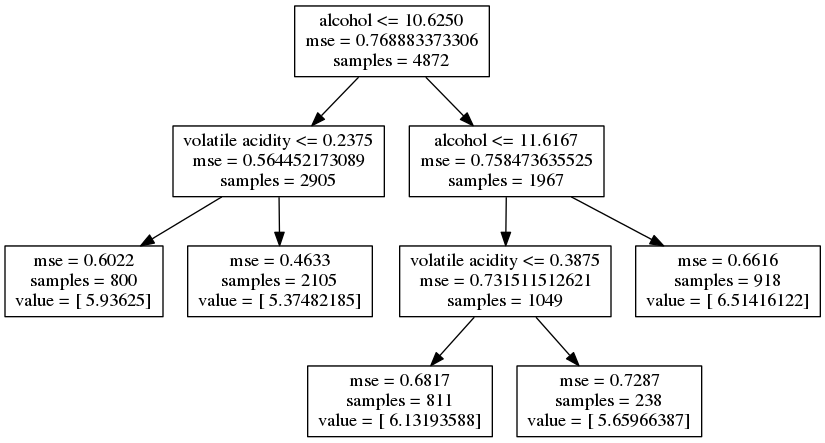
\includegraphics[width=0.8\textwidth]{./figures/wine-tree.png}
\end{figure}

\end{frame}

\begin{frame}
  \frametitle{Strengths and weaknesses}

  \begin{itemize}
    \item {\color{blue} Non-parametric} model

    \vspace{0.25cm}

    \item {\color{blue} Fast} to train ($\Theta(pN\log^2 N)$)

    \vspace{0.25cm}

    \item Easily {\color{blue} interpretable}

    \vspace{0.25cm}

    \item {\color{blue} Low bias}, but usually {\color{red} high variance}\\
        \begin{itemize}
            \item Solution: {\it Combine the predictions of several randomized trees into a single model.}
        \end{itemize}
  \end{itemize}
\end{frame}


% Forests and boosting ========================================================

\section{Random Forests}

\begin{frame}
    \frametitle{Random Forests}

    \begin{figure}
        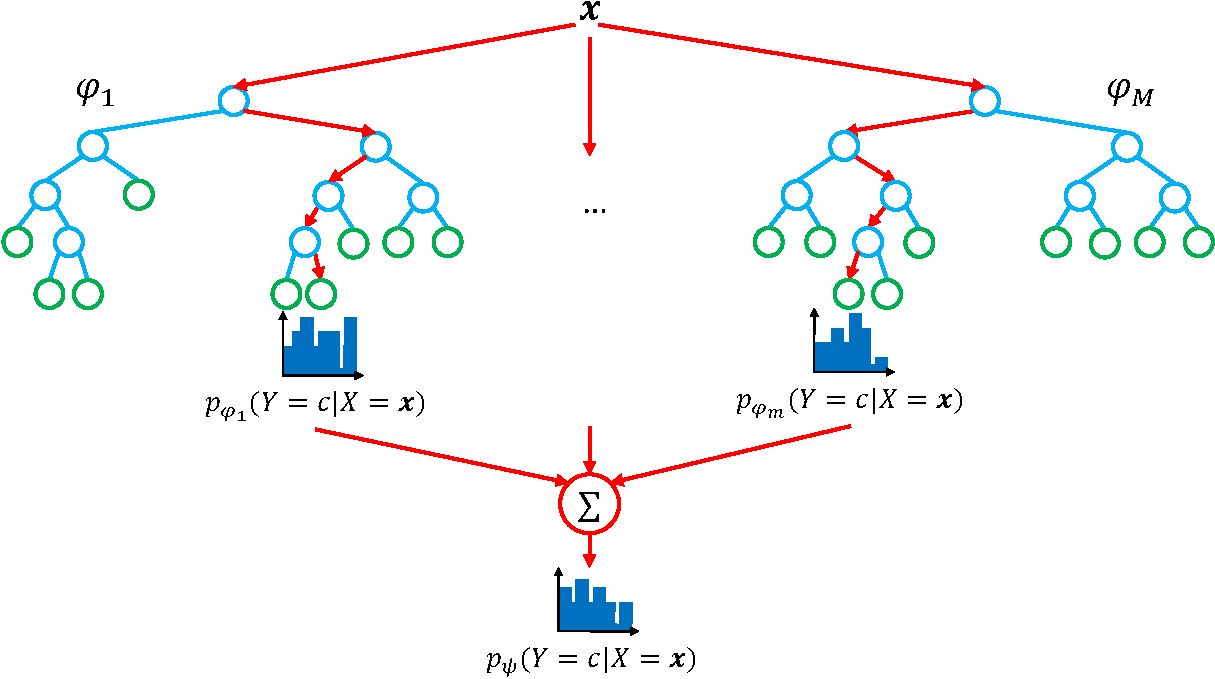
\includegraphics[scale=0.5]{./figures/forest.pdf}
    \end{figure}

    Randomization

    \vspace{0.1cm}

    {\scriptsize
    \begin{tabular}{lll}

    \textbullet\hspace*{0.1cm} Bootstrap samples & \multirow{2}{*}{{\LARGE \}} {\color{blue} Random Forests}} & \\
    \textbullet\hspace*{0.1cm}  Random selection of $K \leq p$ split variables && \multirow{2}{*}{{\LARGE \}} {\color{blue} Extra-Trees}} \\
    \textbullet\hspace*{0.1cm}  Random selection of the threshold  & \\
    \end{tabular}}
\end{frame}

\begin{frame}{Bias and variance}
    \begin{figure}
        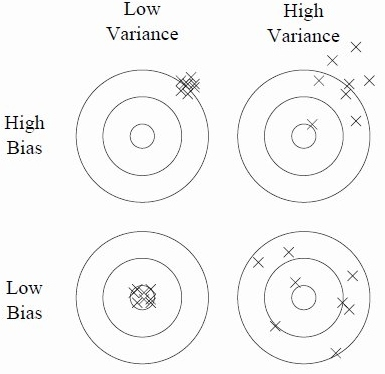
\includegraphics[scale=0.7]{./figures/bias-variance-darts.jpg}
    \end{figure}
\end{frame}

\begin{frame}{Bias-variance decomposition}

{\bf Theorem.}
For the squared error loss, the bias-variance decomposition of the expected
generalization error $\mathbb{E}_{\cal L} \{ Err( \psi_{{\cal L},\theta_1,\dots,\theta_M}(\mathbf{x}))
\}$ at $X=\mathbf{x}$ of an ensemble of $M$ randomized models $\varphi_{{\cal L},\theta_m}$ is
\begin{equation*}
\mathbb{E}_{\cal L} \{ Err(\psi_{{\cal L},\theta_1,\dots,\theta_M}(\mathbf{x})) \} = \text{noise}(\mathbf{x}) + \text{bias}^2(\mathbf{x}) + \text{var}(\mathbf{x}),
\end{equation*}
where
\begin{align*}
\text{noise}(\mathbf{x}) &= Err(\varphi_B(\mathbf{x})), \\
\text{bias}^2(\mathbf{x}) &= (\varphi_B(\mathbf{x}) - \mathbb{E}_{{\cal L},\theta} \{ \varphi_{{\cal L},\theta}(\mathbf{x}) \} )^2, \\
\text{var}(\mathbf{x}) &= \rho(\mathbf{x}) \sigma^2_{{\cal L},\theta}(\mathbf{x}) + \frac{1 - \rho(\mathbf{x})}{M} \sigma^2_{{\cal L},\theta}(\mathbf{x}).
\end{align*}

and where $\rho(\mathbf{x})$ is the Pearson correlation coefficient between
the predictions of two randomized trees built on the same learning set.

\end{frame}


\begin{frame}{Diagnosing the generalization error of random forests}

\begin{itemize}
\item Bias: {\color{blue} Identical} to the bias of a single randomized tree.
\item Variance: $\text{var}(\mathbf{x}) = \rho(\mathbf{x}) \sigma^2_{{\cal L},\theta}(\mathbf{x}) + \frac{1 - \rho(\mathbf{x})}{M} \sigma^2_{{\cal L},\theta}(\mathbf{x})$\\
As $M \to \infty$, {\color{red} $\text{var}(\mathbf{x}) \to \rho(\mathbf{x}) \sigma^2_{{\cal L},\theta}(\mathbf{x})$}
  \begin{itemize}
    \item The stronger the randomization, $\rho(\mathbf{x}) \to 0$, $\text{var}(\mathbf{x}) \to 0$.
    \item The weaker the randomization, $\rho(\mathbf{x}) \to 1$, $\text{var}(\mathbf{x}) \to \sigma^2_{{\cal L},\theta}(\mathbf{x})$
  \end{itemize}
\end{itemize}

\vspace{1cm}

{\bf Bias-variance trade-off.} Randomization increases bias but makes it
possible to reduce the variance of the corresponding ensemble model. The crux
of the problem is to {\color{red} find the right trade-off}.

\end{frame}


\begin{frame}[fragile]
\frametitle{Tuning randomness in \texttt{sklearn.ensemble}}

{\scriptsize
\begin{pythoncode}
from sklearn.ensemble import RandomForestRegressor, ExtraTreesRegressor
from sklearn.cross_validation import ShuffleSplit
from sklearn.learning_curve import validation_curve

# Validation of max_features, controlling randomness in forests
param_name = "max_features"
param_range = range(1, X.shape[1]+1)

for Forest, color, label in [(RandomForestRegressor, "g", "RF"),
                             (ExtraTreesRegressor, "r", "ETs")]:
    _, test_scores = validation_curve(
        Forest(n_estimators=100, n_jobs=-1), X, y,
        cv=ShuffleSplit(n=len(X), n_iter=10, test_size=0.25),
        param_name=param_name, param_range=param_range,
        scoring="mean_squared_error")
    test_scores_mean = np.mean(-test_scores, axis=1)
    plt.plot(param_range, test_scores_mean, label=label, color=color)

plt.xlabel(param_name)
plt.xlim(1, max(param_range))
plt.ylabel("MSE")
plt.legend(loc="best")
plt.show()
\end{pythoncode}
}

\end{frame}


\begin{frame}[fragile]
\frametitle{Tuning randomness in \texttt{sklearn.ensemble}}

    \begin{figure}
        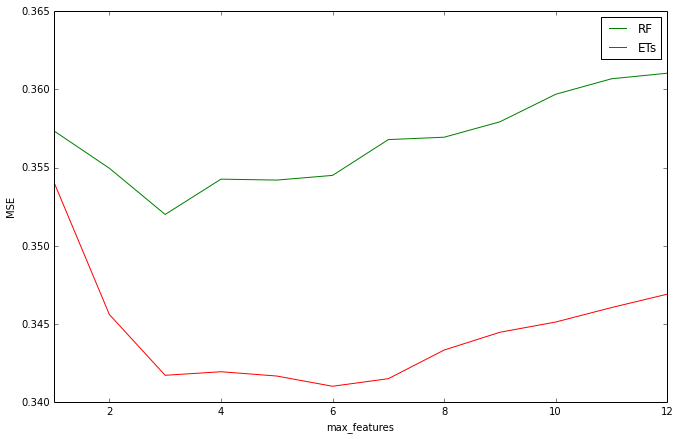
\includegraphics[width=0.9\textwidth]{./figures/randomness.png}
    \end{figure}

Best-tradeoff: ExtraTrees, for \texttt{max\_features=6}.

\end{frame}


\begin{frame}
  \frametitle{Strengths and weaknesses}
\end{frame}


% Forests and boosting ========================================================

\section{Boosting}

\begin{frame}
  \frametitle{Gradient Boosted Regression Trees}
\end{frame}

\begin{frame}
  \frametitle{Strengths and weaknesses}
\end{frame}

% Framework (loss function, regularization, etc)


% Reading tree leaves =========================================================

\section{Reading tree leaves}

\begin{frame}
  \frametitle{Variable importances}
\end{frame}

\begin{frame}
  \frametitle{Partial dependence plots}
\end{frame}

\begin{frame}
  \frametitle{Outlier detection}
\end{frame}

\begin{frame}
  \frametitle{Embedding}
\end{frame}



% Summary =================================================================

% strong points and weaknesses
% going further


\section{Summary}

\begin{frame}
  \frametitle{Summary}
\end{frame}

\begin{frame}
\begin{center}
{\Huge  Questions?}
\end{center}
\end{frame}

\end{document}
